\documentclass{standalone}
\usepackage{tikz}
\usepackage{pgfplots}
\pgfplotsset{compat=1.18}

\begin{document}

% Bit prediction
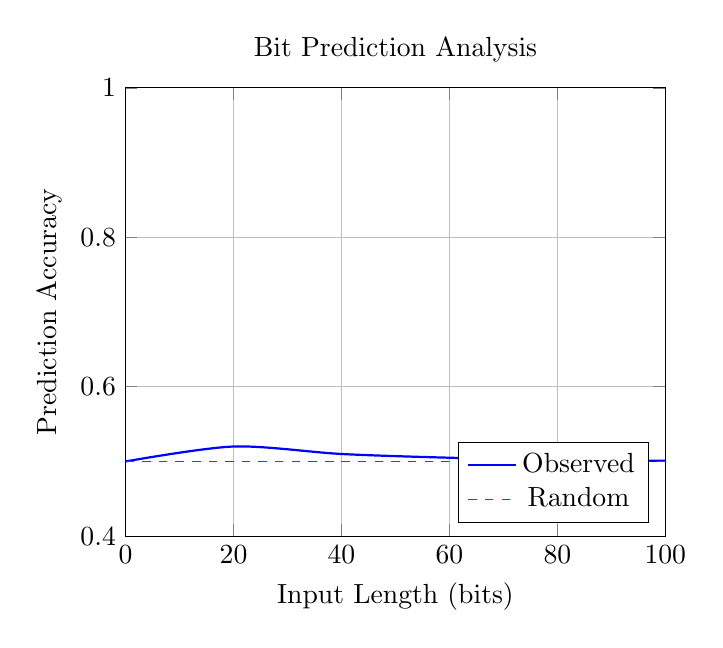
\begin{tikzpicture}
\begin{axis}[
    xlabel={Input Length (bits)},
    ylabel={Prediction Accuracy},
    title={Bit Prediction Analysis},
    grid=major,
    xmin=0, xmax=100,
    ymin=0.4, ymax=1.0,
    legend pos=south east
]

\addplot[smooth, thick, blue] coordinates {
    (0, 0.5)
    (20, 0.52)
    (40, 0.51)
    (60, 0.505)
    (80, 0.502)
    (100, 0.501)
};

\addplot[smooth, dashed, red] coordinates {
    (0, 0.5)
    (20, 0.5)
    (40, 0.5)
    (60, 0.5)
    (80, 0.5)
    (100, 0.5)
};

\legend{Observed, Random}
\end{axis}
\end{tikzpicture}

% Vertical structure
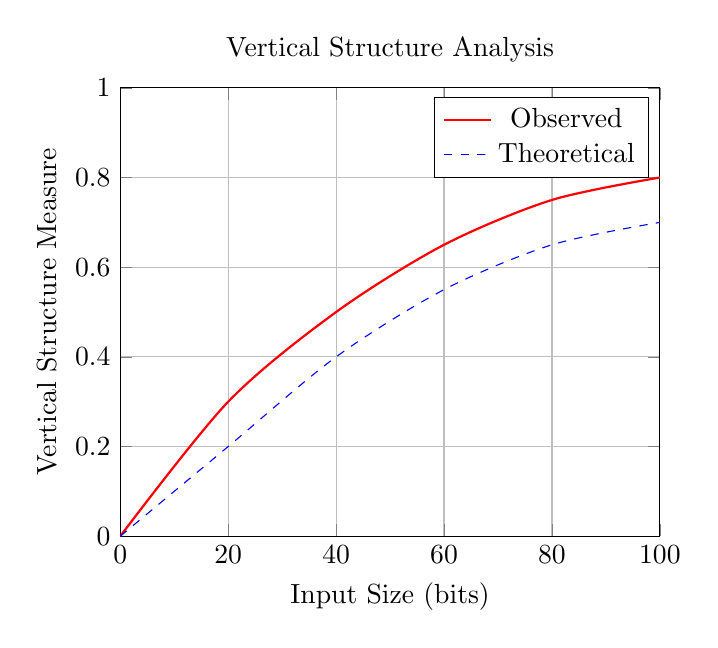
\begin{tikzpicture}
\begin{axis}[
    xlabel={Input Size (bits)},
    ylabel={Vertical Structure Measure},
    title={Vertical Structure Analysis},
    grid=major,
    xmin=0, xmax=100,
    ymin=0, ymax=1
]
\addplot[smooth, thick, red] coordinates {
    (0, 0)
    (20, 0.3)
    (40, 0.5)
    (60, 0.65)
    (80, 0.75)
    (100, 0.8)
};
\addplot[smooth, dashed, blue] coordinates {
    (0, 0)
    (20, 0.2)
    (40, 0.4)
    (60, 0.55)
    (80, 0.65)
    (100, 0.7)
};
\legend{Observed, Theoretical}
\end{axis}
\end{tikzpicture}

% Compression distribution
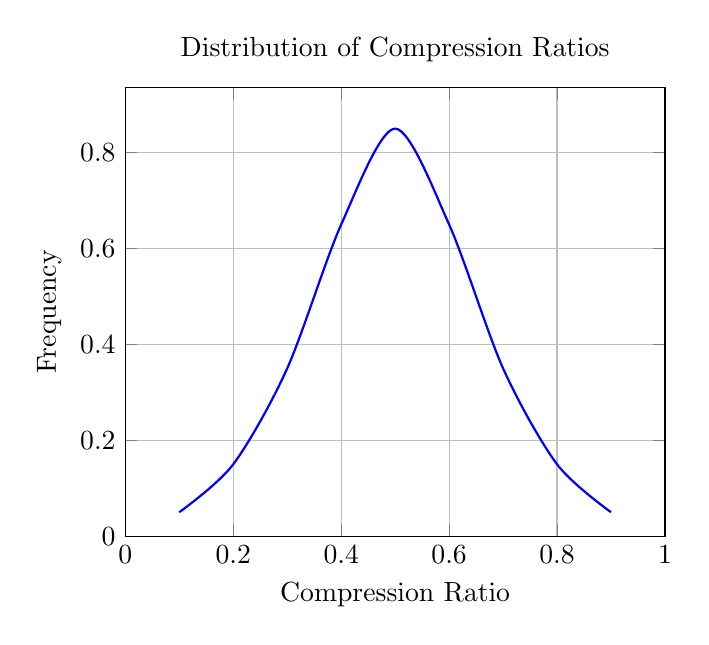
\begin{tikzpicture}
\begin{axis}[
    xlabel={Compression Ratio},
    ylabel={Frequency},
    title={Distribution of Compression Ratios},
    grid=major,
    xmin=0, xmax=1,
    ymin=0
]
\addplot[smooth, thick, blue] coordinates {
    (0.1, 0.05)
    (0.2, 0.15)
    (0.3, 0.35)
    (0.4, 0.65)
    (0.5, 0.85)
    (0.6, 0.65)
    (0.7, 0.35)
    (0.8, 0.15)
    (0.9, 0.05)
};
\end{axis}
\end{tikzpicture}

% Tau distribution
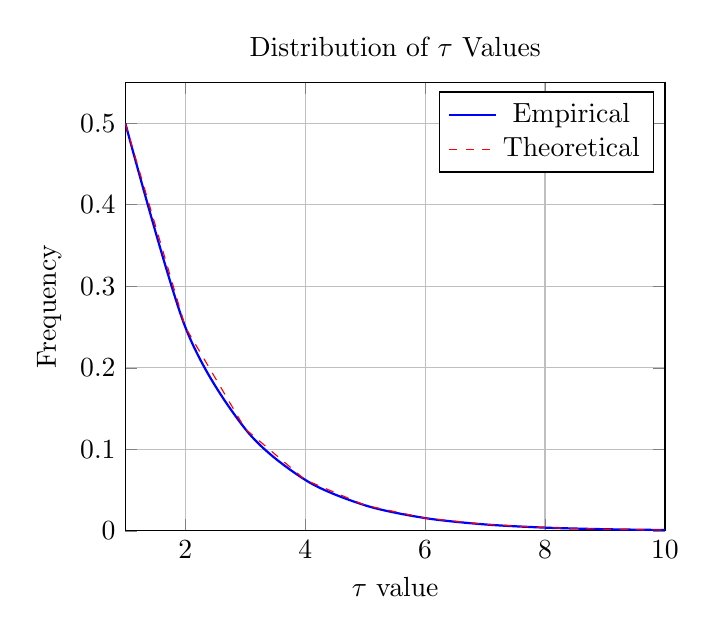
\begin{tikzpicture}
\begin{axis}[
    xlabel={$\tau$ value},
    ylabel={Frequency},
    title={Distribution of $\tau$ Values},
    grid=major,
    xmin=1, xmax=10,
    ymin=0
]
\addplot[smooth, thick, blue] coordinates {
    (1, 0.5)
    (2, 0.25)
    (3, 0.125)
    (4, 0.0625)
    (5, 0.03125)
    (6, 0.015625)
    (7, 0.0078125)
    (8, 0.00390625)
    (9, 0.001953125)
    (10, 0.0009765625)
};
\addplot[dashed, red] coordinates {
    (1, 0.5)
    (2, 0.25)
    (3, 0.125)
    (4, 0.0625)
    (5, 0.03125)
    (6, 0.015625)
    (7, 0.0078125)
    (8, 0.00390625)
    (9, 0.001953125)
    (10, 0.0009765625)
};
\legend{Empirical, Theoretical}
\end{axis}
\end{tikzpicture}

% Entropy reduction
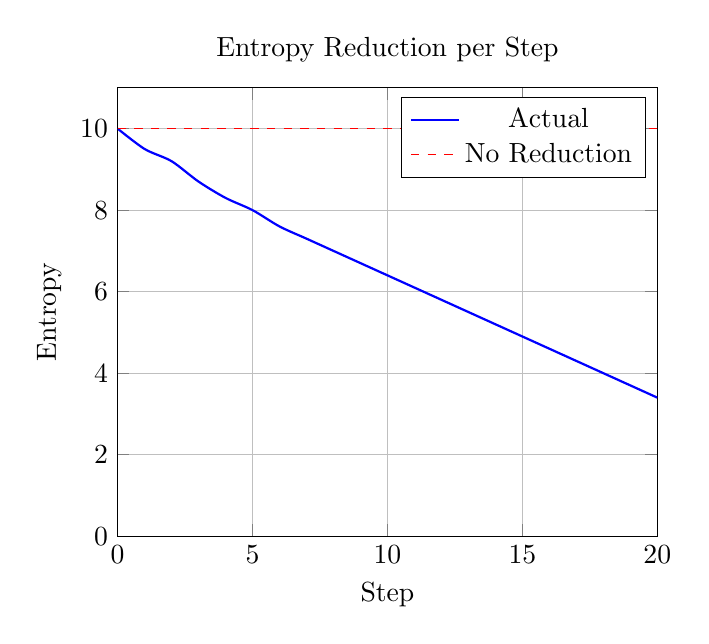
\begin{tikzpicture}
\begin{axis}[
    xlabel={Step},
    ylabel={Entropy},
    title={Entropy Reduction per Step},
    grid=major,
    xmin=0, xmax=20,
    ymin=0
]
\addplot[smooth, thick, blue] coordinates {
    (0, 10)
    (1, 9.5)
    (2, 9.2)
    (3, 8.7)
    (4, 8.3)
    (5, 8.0)
    (6, 7.6)
    (7, 7.3)
    (8, 7.0)
    (9, 6.7)
    (10, 6.4)
    (11, 6.1)
    (12, 5.8)
    (13, 5.5)
    (14, 5.2)
    (15, 4.9)
    (16, 4.6)
    (17, 4.3)
    (18, 4.0)
    (19, 3.7)
    (20, 3.4)
};
\addplot[dashed, red] coordinates {
    (0, 10)
    (20, 10)
};
\legend{Actual, No Reduction}
\end{axis}
\end{tikzpicture}

% Transformation phases
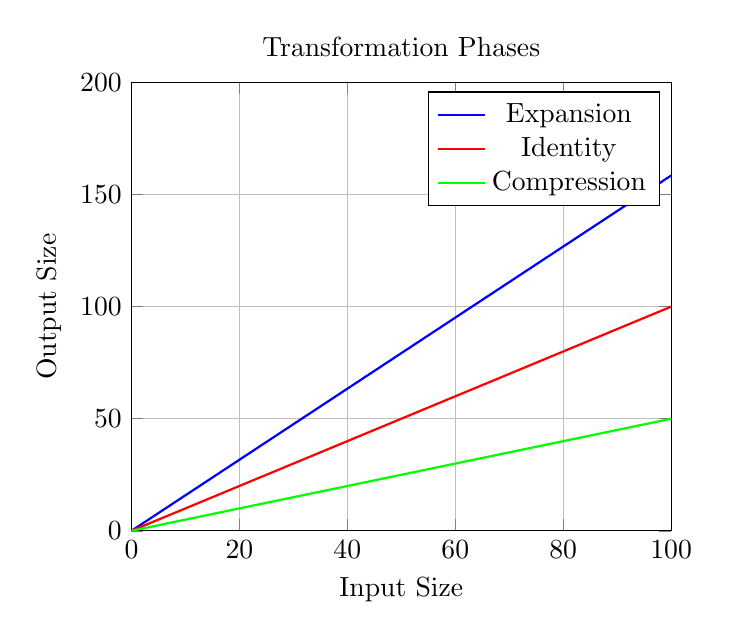
\begin{tikzpicture}
\begin{axis}[
    xlabel={Input Size},
    ylabel={Output Size},
    title={Transformation Phases},
    grid=major,
    xmin=0, xmax=100,
    ymin=0, ymax=200
]
\addplot[thick, blue] coordinates {
    (0, 0)
    (20, 31.7)
    (40, 63.4)
    (60, 95.1)
    (80, 126.8)
    (100, 158.5)
};
\addplot[thick, red] coordinates {
    (0, 0)
    (20, 20)
    (40, 40)
    (60, 60)
    (80, 80)
    (100, 100)
};
\addplot[thick, green] coordinates {
    (0, 0)
    (20, 10)
    (40, 20)
    (60, 30)
    (80, 40)
    (100, 50)
};
\legend{Expansion, Identity, Compression}
\end{axis}
\end{tikzpicture}

% Bit patterns
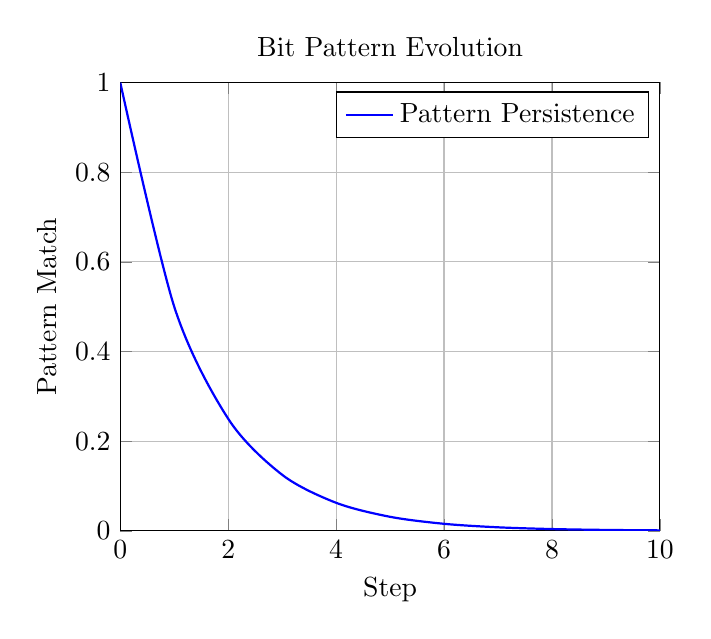
\begin{tikzpicture}
\begin{axis}[
    xlabel={Step},
    ylabel={Pattern Match},
    title={Bit Pattern Evolution},
    grid=major,
    xmin=0, xmax=10,
    ymin=0, ymax=1
]
\addplot[smooth, thick, blue] coordinates {
    (0, 1.0)
    (1, 0.5)
    (2, 0.25)
    (3, 0.125)
    (4, 0.0625)
    (5, 0.03125)
    (6, 0.015625)
    (7, 0.0078125)
    (8, 0.00390625)
    (9, 0.001953125)
    (10, 0.0009765625)
};
\legend{Pattern Persistence}
\end{axis}
\end{tikzpicture}

% Compression ratio
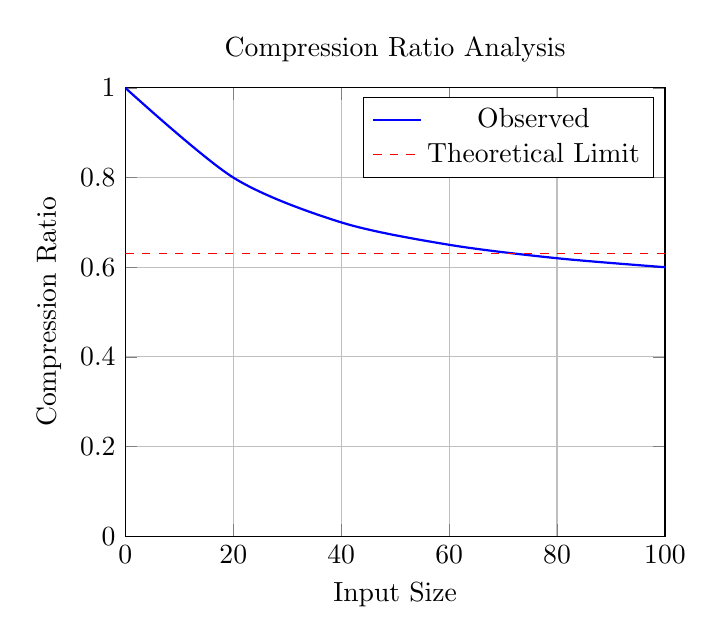
\begin{tikzpicture}
\begin{axis}[
    xlabel={Input Size},
    ylabel={Compression Ratio},
    title={Compression Ratio Analysis},
    grid=major,
    xmin=0, xmax=100,
    ymin=0, ymax=1
]
\addplot[smooth, thick, blue] coordinates {
    (0, 1.0)
    (20, 0.8)
    (40, 0.7)
    (60, 0.65)
    (80, 0.62)
    (100, 0.6)
};
\addplot[dashed, red] coordinates {
    (0, 0.63)
    (100, 0.63)
};
\legend{Observed, Theoretical Limit}
\end{axis}
\end{tikzpicture}

\end{document} 